\documentclass{easychair}

% \usepackage{doc}
\usepackage{setspace}
\usepackage{verbatim}

%----Making things more compact
\newcommand{\smalltt}[1]{\small \texttt{#1}}
\newenvironment{packed_itemize}{
\vspace*{-0.2em}
\begin{itemize}
\setlength{\partopsep}{0pt}
\setlength{\itemsep}{1pt}
\setlength{\parskip}{0pt}
\setlength{\parsep}{0pt}
}{\end{itemize}}
\newenvironment{packed_enumerate}{
\vspace*{-0.2em}
\begin{enumerate}
\setlength{\partopsep}{0pt}
\setlength{\itemsep}{1pt}
\setlength{\parskip}{0pt}
\setlength{\parsep}{0pt}
}{\end{enumerate}}
% \renewcommand{\textfraction}{0.07}
% \renewcommand{\topfraction}{0.9}
% \renewcommand{\bottomfraction}{0.9}
% \renewcommand{\floatpagefraction}{0.66}
% \setlength{\floatsep}{2.0pt plus 2.0pt minus 2.0pt}
% \setlength{\textfloatsep}{5.0pt plus 2.0pt minus 0.0pt}

%----For Alex's proof stuff
\usepackage{amsmath,amssymb,amsthm}
\newtheorem*{lemma}{Lemma}
\newtheorem*{theorem}{Theorem}
\newcommand{\true}{{\mathit{true}}}
\newcommand{\false}{{\mathit{false}}}

\title{The New TPTP Format for \\ Tarskian and Kripke Interpretations}

\author{
  Geoff Sutcliffe\inst{1}
\and
  Alexander Steen\inst{2}
\and
  Pascal Fontaine\inst{3}
}

\institute{
  University of Miami,
  Miami, USA\\
  \email{geoff@cs.miami.edu,jam771@miami.edu}
\and
  University of Greifswald,
  Greifswald, Germany\\
  \email{alexander.steen@uni-greifswald.de}
\and
  University of Li{\`e}ge,
  Li{\`e}ge, Belgium\\
  \email{Pascal.Fontaine@uliege.be}
}

\authorrunning{Sutcliffe, Steen, Fontaine}
\titlerunning{TPTP Interpretations}

\begin{document}
\maketitle

%--------------------------------------------------------------------------------------------------
\begin{abstract}
This paper describes a new format for representing Tarskian and Kripke interpretations.
%formulae in untyped and typed first-order logic, using the TPTP TF0 language.
\end{abstract}
%--------------------------------------------------------------------------------------------------
\section{Introduction}
\label{Introduction}

Historically, Automated Theorem Proving (ATP) has, as the name suggests, focused largely on the
task of proving theorems from axioms -- the derivation of conclusions that follow inevitably 
from known facts \cite{RV01-HAR}.
The axioms and conjecture to be proved (and hence become a theorem) are written in an 
appropriately expressive logic, and the proofs are often similarly written in logic \cite{SS+06}.
% In this work simply-typed first-order logic in the form of \cite{Wal83,Sch85,Coh87},
% whose expressive power is sufficient for a wide range of topics \cite{Sut17}, is used
In the last two decades the converse task of disproving conjectures, i.e., proving that a 
conjecture is not a theorem of the axioms, has become increasingly important.
This process depends on finding an {\em interpretation}, i.e., a structure that maps terms 
to domain elements and formulae to truth values.
An interpretation that maps a formula to {\em true} is a {\em model} of the formula.
A conjecture is disproved by finding an interpretation that is a model of the axioms, but 
is not a model of the conjecture, aka a {\em countermodel} for the conjecture.
A salient application area that harnesses this form of ATP is verification \cite{DKW08},
where a countermodel is used to pinpoint the reason why a proof obligation fails, and
correspondingly points to the location of the fault in the system being verified.
Other applications of model finding include checking the consistency of an axiomatization 
\cite{SS+17}, and finding a solution to a problem that is coded as a model finding problem 
\cite{Win82}.

The TPTP World \cite{Sut17} (\href{https://www.tptp.org}{\tt www.tptp.org}) is a well established 
infrastructure that supports research, development, and deployment of Automated Theorem Proving 
(ATP) systems.
Various parts of the TPTP World have been deployed in a range of applications,
in both academia and industry.
The TPTP World includes the TPTP problem library \cite{Sut09}, 
the TSTP solution library \cite{Sut10}, 
tools and services for processing ATP problems and solutions \cite{Sut10}, 
it supports the CADE ATP System Competition (CASC) \cite{Sut16}.
Most relevant to this work the TPTP World provides formats for writing ATP problems, 
derivations, and interpretations \cite{SS+06,Sut08-KEAPPA}.
This work describes the new TPTP format for interpretations.
The new format replaces the old format for finite interpretations \cite{SS+06}, which has 
served the community adequately for almost 20 years, and is output by several ATP systems, e.g., 
Paradox \cite{CS03}, FMDarwin \cite{BF+06}, Vampire \cite{KV13}.

\paragraph{Related Work:}
The SMT-LIB standard \cite{BFT17} defines a format for model output, and commands to inspect 
models.  
SAT solvers generally output models as specified by the SAT competitions \cite{JL+12}, in a 
simple format similar to the DIMACS input format \cite{Bab93}.
iProver, DIGs.
Some individual model finding systems have defined their own formats for models, e.g., the 
output formats of Nitpick and Z3 \cite{dMB08}.
% +++
% Nikolaj says ...
% Z3 It produces models that define functions by expressions. For example a model of succ is 
% Succ(x) =X+ 1
% Works when domain is integer. Currently z3 does not implement infinite models for uninterpreted sorts. I would probably support infinite sorts by creating injection into an algebraic datatype and then support models that can be expressed over ADT.
% See also https://microsoft.github.io/z3guide/docs/logic/Quantifiers
% +++

This paper is organized as follows:
Section~\ref{TPTP} introduces the TPTP World which provides the framework and languages used
in this research.
Section~\ref{Interpretations} discusses the nature of interpretations, considering what is
needed from interpretations, and the various forms that interpretations can take.
Section~\ref{NewTarskian} defines the new format for Tarskian interpretations, and
Section~\ref{NewKripke} does the same for Kripke interpretations.
Section~\ref{Tools} reviews some TPTP World tools for examining and manipulating interpretations.
Section~\ref{Conclusion} concludes and discusses plans for future work.

%--------------------------------------------------------------------------------------------------
\section{The TPTP World and Languages}
\label{TPTP}

The TPTP language \cite{Sut22-IGPL} is one of the keys to the success of the TPTP World.
The language is used for writing both problems and solutions,
which enables convenient communication between systems. 
% It also enables tool exchange, tool integration, and comparable experimental results.
Originally the TPTP World supported only first-order clause normal form (CNF)
\cite{SS98-JAR}.
Over the years full first-order form (FOF)
\cite{Sut09}, 
typed first-order form (TFF)
\cite{SS+12,BP13-TFF1}, 
typed extended first-order form (TXF)
\cite{SK18}, 
typed higher-order form (THF)
\cite{SB10,KSR16}, 
and non-classical forms (NTF)
\footnote{%
There are many ``non-classical logics'', including multi-valued logics \cite{Aug17},
paraconsistent logics \cite{Pri02}, relevance logics \cite{AB75}, etc.
In this work we are interested in those that admit Kripke interpretation \cite{Kri63},
e.g., modal logics \cite{BBW06}.}
\cite{SF+22} 
have been added.
A general principle of the TPTP language is ``we provide the syntax, you provide the semantics''.
As such, there is no a priori commitment to any semantics for the languages, although in almost 
all cases the intended logic and semantics are well known.
All the typed forms include constructs for arithmetic.
TF0 \cite{SS+12}, the monomorphic subform of TFF, is used in this work (see Section~\ref{TF0}).

The top level building blocks of the TPTP language are {\em annotated formulae}.
An annotated formula has the form:\\
\hspace*{0.5cm}{\em language}{\tt (}{\em name}{\tt ,}
{\em role}{\tt ,}
{\em formula}{\tt ,}
{\em source}{\tt ,}
{\em useful\_info}{\tt )}\\
The {\em language}s supported are {\smalltt{cnf}} (clause normal form), {\smalltt{fof}}
(first-order form), {\smalltt{tff}} (typed first-order form), and {\smalltt{thf}}
(typed higher-order form).
The {\em role}, e.g., {\smalltt{axiom}}, {\smalltt{lemma}}, {\smalltt{conjecture}},
defines the use of the formula in an ATP system.
In a {\em formula}, terms and atoms follow Prolog conventions
-- functions and predicates start with a lowercase letter or are {\tt '}single quoted{\tt '}, and 
variables start with an uppercase letter.
The language also supports interpreted symbols, which either start with a {\tt \$}, e.g., 
the truth constants {\smalltt{\$true}} and {\smalltt{\$false}}, or are composed of 
non-alphabetic characters, e.g., integer/rational/real numbers such as 27, 43/92, -99.66.
The logical connectives in the TPTP language are
{\tt !}, {\tt ?}, {\tt {\raisebox{0.4ex}{\texttildelow}}}, {\tt |}, {\tt \&}, {\tt =>}, {\tt <=},
{\tt <=>}, and {\tt <{\raisebox{0.4ex}{\texttildelow}}>},
for the mathematical connectives
$\forall$, $\exists$, $\neg$, $\vee$, $\wedge$, $\Rightarrow$, $\Leftarrow$, $\Leftrightarrow$, 
and $\oplus$ respectively.
Equality and inequality are expressed as the infix operators {\tt =} and {\tt !=}.
The {\em source} and {\em useful\_info} are optional.
Annotated formulae (using TF0) can be seen in 
Figures~\ref{TF0FiniteProblem}-\ref{TF0InfiniteVerification}.

%--------------------------------------------------------------------------------------------------
\subsection{The TF0 Language}
\label{TF0}

% is a typed first-order language extended with FOOL logic constructs.
TF0 is a typed first-order language.
The TF0 types are
(i)~the predefined types {\smalltt{\$i}} for individuals and {\smalltt{\$o}} for booleans; 
(ii)~the predefined arithmetic types {\smalltt{\$int}}, {\smalltt{\$rat}}, and {\smalltt{\$real}}; 
(iii)~user-defined types declared to be of the kind {\smalltt{\$tType}}.
Every symbol is declared with a type signature:
(i)~individual types for variables;
(ii)~function types from non-boolean argument types to a non-boolean result type;
(iii)~predicate types from non-boolean argument types to a boolean result.
The equality predicates {\tt =} and {\tt !=} are ad hoc polymorphic over all types. 
Arithmetic predicates and functions are ad hoc polymorphic over the arithmetic types.
% TX0 formulae are those of first-order logic, extended to allow boolean variables and terms.
% TX0 additionally supports tuples, conditional expressions, and let expressions, but they are
% not used in this paper (see \cite{SK18} for the details).
Figures~\ref{TF0FiniteProblem}~and~\ref{TF0InfiniteProblem} are examples of problems in TF0.  Their associated (counter)models are discussed in Section~\ref{Interpretations}.

\begin{figure}[htbp]
\small
\setstretch{0.9}
\verbatiminput{TFF_Finite.p}
\caption{A TF0 problem (with a finite countermodel)\\
{\footnotesize \url{https://raw.githubusercontent.com/GeoffsPapers/ModelVerificationLPAR/master/TFF_Finite.p}}}
\label{TF0FiniteProblem}
\end{figure}

\begin{figure}[htbp]
\small
\setstretch{0.9}
\verbatiminput{TFF_Infinite.p}
\caption{A TF0 problem (with an infinite model)\\
{\footnotesize \url{https://raw.githubusercontent.com/GeoffsPapers/ModelVerificationLPAR/master/TFF_Infinite.p}}}
\label{TF0InfiniteProblem}
\end{figure}

%--------------------------------------------------------------------------------------------------
\section{Interpretations}
\label{Interpretations}

A Tarskian-style interpretation \cite{TV56} of formulae in typed first-order logic consists of a 
non-empty domain of unequal elements for each type used in the formulae (just one domain for 
untyped logic), and interpretations of the function and predicate symbols with respect to the 
domains \cite{Hun96,Gal15}.
$I \vdash \Phi$ means the interpretation $I$ is a model of the formula $\Phi$.
An interpretation can normally interpret all expressions that can be written in the language of 
the formulae, but in some circumstances an interpretation can interpret only (at least) the given 
formulae, e.g., \cite{BSW23}; such an interpretation is a {\em partial interpretation}.

The domains of an interpretation may be finite or infinite.
Interpretations with only finite domains are called {\em finite interpretations}, and
interpretations with one or more infinite domains are called {\em infinite interpretations}.
Finite domains are commonly explicitly enumerated, but can also take other forms, e.g., the 
finite Herbrand Universe of a Herbrand interpretation \cite{Her30}.
Infinite domains can take several forms, including being implicitly specified (e.g., some set
of algebraic numbers, such as the integers), explicitly generated (e.g., terms representing 
Peano numbers), and the infinite Herbrand Universe of a Herbrand interpretation.

In addition to Tarskian-style interpretations that provide explicit symbol interpretation, 
a Herbrand interpretation can also be embodied in a saturation \cite{BG+01},
i.e., a fixed point for a set of clauses at which further application of a complete inference 
system does not generate any new clauses.
This approach is adopted in saturation-based ATP systems such as E \cite{SCV19},
Prover9 \cite{McC-Prover9-URL}, Vampire, and Zipperposition \cite{VB+21}.
While the domain of a saturation is known to be the Herbrand Universe, there is no explicit
symbol interpretation that can be used constructively by users.
Saturations are thus a less useful form of interpretation.
This work considers only Tarskian-style interpretations.

The notions of interpretations, models, partial interpretations, finite interpretations,
Herbrand interpretations, etc., are captured in the SZS ontologies \cite{Sut08-KEAPPA}, as
updated at 
{\smalltt{\url{https://www.tptp.org/cgi-bin/SeeTPTP?Category=Documents&File=SZSOntology}}}

%--------------------------------------------------------------------------------------------------
\subsection{Representing Interpretations in TF0}
\label{InterpretationsTF0}

As noted in Section~\ref{Introduction}, a TPTP format for interpretations with finite domains 
has previously been defined, and was been adopted by some ATP systems.
Recently the need for a format for interpretations with infinite domains, and for a format for 
Kripke interpretations \cite{Kri63} of formulae written in the NTF language \cite{SF+22}, 
led to the development of a new TPTP format for interpretations.
The changes allow for multiple interpretations to be given in a single file, which, in the case 
of typed logics, share type declarations.
The underlying principle is unchanged: interpretations are represented as formulae.
This provides the basis for verification of models, as explained in Section~\ref{Verification}.

The new format uses an {\em interpretation formula}. 
Examples of interpretation formulae can be seen in Figures~\ref{TF0FiniteInterpretation}
and~\ref{TF0InfiniteInterpretation}, illustrating the components described next. 
An interpretation formula is a conjunction of three components:
\begin{packed_itemize}
\item a conjunction of the domain specifications for the types in the given formulae:
      for each type a {\em type-promotion} function that converts domain elements to terms is
      used to keep the interpretation formula well-typed; each domain specification is a 
      conjunction of:
      \begin{packed_itemize}
      \item the domain type, by a formula that makes the type-promotion function a surjection 
            (unless it is unnecessary because the type is defined and is the same as the type in 
            the given formulae, e.g., both are {\smalltt{\$int}});
      \item the domain elements (unless implicit from their defined type): if the domain is
            finite this is a universally quantified disjunction of equalities whose right-hand 
            sides are the terms; if the domain is infinite an existentially quantified formula 
            that captures an infinite disjunction of equalities is used, e.g., for terms 
            representing Peano numbers as the domain elements:\\
            \hspace*{0.5cm}$\forall I{:}peano\;((I = zero) \vee \exists P{:}peano\;(I = s(P)))$;
%            \smalltt{! [I: peano] : ( I = zero | ? [P: peano] : I = s(P) )};
      \item specification of the distinctness of the domain elements (unless implicit from their
            defined type);
      \item a formula making the type-promotion function an injection,
            % (unless the type of the domain is the same as the type in the formula), 
            which together with the surjectivity makes it a bijection.
      \end{packed_itemize}
\item interpretation of the function symbols, as equalities whose left-hand sides are 
      formed from symbols applied to type-promoted domain elements, and whose right-hand sides 
      are type-promoted domain elements;
\item interpretation of the predicate symbols, as literals formed from symbols applied
      to type-promoted domain elements; positive literals are {\em true} and negative literals 
      are {\em false}.
\end{packed_itemize}
The interpretation formula is preceded by the necessary type declarations:
\begin{packed_itemize}
\item the types in the given formulae (except defined types, e.g., {\smalltt{\$int}});
\item the types of the domains (except defined types);
\item the types of type-promotion functions;
\item the types of the domain elements.
\end{packed_itemize}
% \vspace*{-0.4em}
This representation is also directly usable for untyped first-order logic, where all terms in 
the given formulae and the interpretation formula are of the same type – ``individuals''. 
This obviates the need for type considerations, in particular type-promotion functions are not 
needed.

Figure~\ref{TF0FiniteInterpretation} is a TF0 interpretation with finite domains -- it is a 
countermodel for the problem in Figure~\ref{TF0FiniteProblem}.
The comments show which parts of the formula specify what aspects of the interpretation.
Figure~\ref{TF0InfiniteInterpretation} is a TF0 interpretation with an infinite domain -- it 
is a model for the problem in Figure~\ref{TF0InfiniteProblem}.
Note that in Figure~\ref{TF0InfiniteInterpretation}:
the defined type {\smalltt{\$int}} is the domain type for the formula type 
{\smalltt{person}}, so that there is no specification of the domain elements and their 
distinctness;
universal quantification is used for the interpretation of function and predicate
symbols for an infinite number of argument tuples;
the interpretations of function and predicate symbols is not given for argument 
tuples with negative integers, i.e., this is an example of a partial interpretation.

\begin{figure}[htbp]
\small
\setstretch{0.9}
\verbatiminput{TFF_Finite.s}
\caption{A TF0 interpretation with a finite domain \\
{\footnotesize \url{https://raw.githubusercontent.com/GeoffsPapers/ModelVerificationLPAR/master/TFF_Finite.s}}}
\label{TF0FiniteInterpretation}
\end{figure}

\begin{figure}[htbp]
\small
\setstretch{0.9}
\verbatiminput{TFF_Integer.s}
\caption{A TF0 interpretation with an infinite domain\\
{\footnotesize \url{https://raw.githubusercontent.com/GeoffsPapers/ModelVerificationLPAR/master/TFF_Integer.s}}}
\label{TF0InfiniteInterpretation}
\end{figure}

%--------------------------------------------------------------------------------------------------
\section{Model Verification}
\label{Verification}

ATP systems are complex pieces of software, implementing complex calculi, with the end goal
being a sound implementation of a sound inference system whose output correctly corroborates the
result obtained.
The reality is that the complexity leads to incorrectness, and as such verification of ATP systems'
outputs is necessary. 
For theorem proving this means verifying the proof output \cite{Sut06}, and for model finding 
this means verifying the model output.
In the context of this work the model verification applies to the type declarations and 
the interpretation formula that represent the model found by the ATP system, and
has (at least) the following aspects:
\begin{packed_enumerate}
\item Are the type declarations and interpretation formula syntactically well-formed 
      and semantically well-typed?
\item Is the interpretation formula satisfiable?
\item Does the interpretation formula correctly represent the interpretation found by the 
      ATP system?
\item Is the interpretation represented by the interpretation formula a model for the given 
      formulae?
\end{packed_enumerate}
\noindent
These questions are answered as follows:
\begin{enumerate}
\item This can be confirmed using standard parsing and type checking tools, e.g., \cite{VS06,HR15}.
\item This can be empirically confirmed using a trusted model finder (in the same way the GDV 
      derivation verifier \cite{Sut06} uses the Otter system \cite{McC03-Otter} as a trusted 
      theorem prover).
      Confirming that the interpretation formula is satisfiable is almost certainly much 
      easier than finding the model itself, so the system used to check the satisfiability can 
      be weaker and more trusted than the system that found the model.
\item This cannot be confirmed, as that representation is internal to the ATP system that found
      the model.
\item In this work a ``semantic'' approach is taken, in which the given formulae $\Phi$ are proved 
      from the interpretation formula $\varphi$ using a trusted theorem prover; $\varphi$ is 
      supplied as an axiom, and $\Phi$ as the conjecture to be proved.
      This approach relies on the proof of soundness below, which shows that if $\Phi$ can be 
      proved from $\varphi$ (written $\varphi \models \Phi$), then the interpretation $I$ 
      represented by $\varphi$ is a model of $\Phi$.

      An implementation is available online as the AGMV tool in the SystemOnTSTP \cite{Sut07-CSR} 
      web interface {\smalltt{\url{https://www.tptp.org/cgi-bin/SystemOnTSTP}}}.
      The tool input is the concatenation of the problem and the interpretation.
      Figure~\ref{TF0InfiniteVerification} shows the verification problem for the problem in 
      Figure~\ref{TF0InfiniteProblem} and its model in Figure~\ref{TF0InfiniteInterpretation}.
      The input to verify the finite countermodel in Figure~\ref{TF0FiniteInterpretation}, for the 
      problem in Figure~\ref{TF0FiniteProblem}, is
      {\smalltt{\url{https://raw.githubusercontent.com/GeoffsPapers/ModelVerificationLPAR/master/TFF_Finite.sp.AGMV.p}}}.
\end{enumerate}

\begin{figure}[htbp]
\small
\setstretch{0.9}
\verbatiminput{TFF_Integer.s.p}
\caption{The TF0 verification problem for 
Figures~\ref{TF0InfiniteProblem}~and~\ref{TF0InfiniteInterpretation}\\
{\footnotesize \url{https://raw.githubusercontent.com/GeoffsPapers/ModelVerificationLPAR/master/TFF_Integer.s.p}}}
\label{TF0InfiniteVerification}
\end{figure}

The proof of soundness is given here for a finite interpretation in untyped first-order logic, 
where (as explained in Section~\ref{InterpretationsTF0}) there is no need for type considerations.
The proof for typed first-order logic follows exactly the same pattern, but is technically
complicated due to the introduction of types and type promotion functions.
The extension to infinite domains is quite simple after that, following 
Section~\ref{InterpretationsTF0}.

\paragraph{Proof}
~\\
Let $\Sigma$ be an untyped first-order language:
\begin{packed_itemize}
\item $V_\Sigma$ - The variable symbols, starting in uppercase.
\item $F_\Sigma$ - The function symbols with arity, in the form $f/n$.
\item $P_\Sigma$ - The predicate symbols with arity, in the form $p/n$.
\end{packed_itemize}
The formulae over $\Sigma$, $\mathcal{F}(\Sigma)$, are defined as usual. 

\vspace*{1em}
\noindent
Let $I$ be an interpretation for $\Sigma$:
\begin{packed_itemize}
\item $D_I$ - A finite set of unequal domain elements.
\item $F_I$ - For each $f/n \in F_\Sigma$, a mapping $f_I: D_I^n \mapsto D_I$.
\item $P_I$ - For each $p/n \in P_\Sigma$, a mapping $p_I: D_I^n \mapsto \{\true,\false\}$.
\end{packed_itemize}

\newpage
\noindent
Recalling Section~\ref{InterpretationsTF0}, an interpretation is represented by an 
{\em interpretation formula}, $\varphi$.
Let:
\begin{packed_itemize}
%----Note they do not have to be constants, so I removed "/0"
\item $D_{\varphi}$ be a set of fresh terms $d_{\varphi}$, one for each $d_I \in D_I$
% \item $D_{I \mapsto \varphi_I}$ be the corresponding mapping from $D_I$ to $D_{\varphi_I}$
\item $D_{\varphi \mapsto I}$ be the corresponding mapping from $D_{\varphi}$ to $D_I$
\item $\Sigma_{\varphi}$ be the untyped first-order language:
      \begin{packed_itemize}
      \item $V_{\Sigma_{\varphi}} = V_\Sigma$
      \item $F_{\Sigma_{\varphi}} = F_\Sigma \cup D_{\varphi}$
      \item $P_{\Sigma_{\varphi}} = P_\Sigma$
      \end{packed_itemize}
\item $\varphi \in \mathcal{F}(\Sigma_{\varphi}) = 
D^\vee_{\varphi} \land D^{\neq}_{\varphi} \land F^\wedge_{\varphi} \land 
P^\wedge_{\varphi}$, where:
\begin{equation*}
\begin{split}
D^\vee_{\varphi}   &= \forall X \bigvee_{d_{\varphi} \in D_{\varphi}} \left(X = d_{\varphi} \right) \\
%D^{\neq}_{\varphi} &= \bigwedge_{\substack{d_{\varphi},e_{\varphi} \in D_{\varphi} \\
%                                             d_{\varphi} \neq\; e_{\varphi}}} \left(d_{\varphi} \neq e_{\varphi} \right) \\
D^{\neq}_{\varphi} &= \bigwedge_{\substack{\{d_{\varphi},e_{\varphi}\} \subseteq D_{\varphi} \\
                                           d_{\varphi} \not\equiv e_{\varphi}}} \left(d_{\varphi} \neq e_{\varphi} \right) \\
F^\wedge_{\varphi} &= \bigwedge_{\substack{f \in F_\Sigma,\;f_I \in F_I \\
                                           (\overline{d_{I,i}} \mapsto d_I) \in f_I \\
                                           D_{\varphi \mapsto I}(d_{\varphi,i}) = d_{I,i} \\
                                           D_{\varphi \mapsto I}(d_{\varphi}) = d_I}} 
                                 ( f(\overline{d_{\varphi,i}}) = d_{\varphi} ) \\
P^\wedge_{\varphi} &= \bigwedge_{\substack{p \in P_\Sigma,\;p_I \in P_I \\
                                           (\overline{d_{I,i}} \mapsto \true) \in p_I \\
                                           D_{\varphi \mapsto I}(d_{\varphi,i}) = d_{I,i}}}
                                 p(\overline{d_{\varphi,i}}) \\
              &\wedge \bigwedge_{\substack{p \in P_\Sigma,\;p_I \in P_I \\
                                           (\overline{d_{I,i}} \mapsto \false) \in p_I \\
                                           D_{\varphi \mapsto I}(d_{\varphi,i}) = d_{I,i}}}
                                 \neg p(\overline{d_{\varphi,i}})
\end{split}
\end{equation*}
\end{packed_itemize}
% (Note that we don't need that the $\mathrm{rep}_d$ are pair-wise distinct so far, because our 
% $I^\prime$ does this. For the backwards direction of the Theorem, we might need this.)

\noindent
Let $I_{\varphi}$ be an interpretation for $\Sigma_{\varphi}$:
\begin{packed_itemize}
\item $D_{I_{\varphi}} = D_I$
\item $F_{I_{\varphi}} = F_I \cup D_{\varphi \mapsto I}$
\item $P_{I_{\varphi}} = P_I$
\end{packed_itemize}

\begin{lemma} 
$I_{\varphi} \vdash \varphi$
\end{lemma}
\begin{proof}
To prove $I_{\varphi} \vdash \varphi$, prove
$I_{\varphi} \vdash D^\vee_{\varphi}$,
$I_{\varphi} \vdash D^{\neq}_{\varphi}$,
$I_{\varphi} \vdash F^\wedge_{\varphi}$ and
$I_{\varphi} \vdash P^\wedge_{\varphi}$:
% Each can be proved separately: 
\begin{itemize}
\item For every $d_{I_{\varphi}} \in D_{I_{\varphi}}$, or equivalently $d_I \in D_I$:
      \begin{packed_itemize}
      \item There is a $d_{\varphi} \in D_{\varphi}$ such that 
            $D_{\varphi \mapsto I}(d_{\varphi}) = d_I$
      \item $(X = d_{\varphi}) \in D^\vee_{\varphi}$
      \item With $X$ set to $d_I$ \\
            $I_{\varphi} \vdash (d_I = d_{\varphi})$ iff \\
            $d_I = F_{I_{\varphi}}(d_{\varphi})$ iff \\
            $d_I = D_{\varphi \mapsto I}(d_{\varphi})$ \\
            which is $\true$ from the selection of $d_{\varphi}$
      \end{packed_itemize}
      For every $d_{I_{\varphi}} \in D_{I_{\varphi}}$, with $X$ set to $d_{I_{\varphi}}$, a 
      disjunct in $D^\vee_{\varphi}$ is $\true$, i.e., $I_{\varphi} \vdash D^\vee_{\varphi}$
\newpage
\item For every $(d_{\varphi} \neq e_{\varphi})$ in $D^{\neq}_{\varphi}$:
      \begin{packed_itemize}
      \item $I_{\varphi} \vdash (d_{\varphi} \neq e_{\varphi})$ iff \\
            $F_{I_{\varphi}}(d_{\varphi}) \neq F_{I_{\varphi}}(e_{\varphi})$ iff \\
            $D_{\varphi \mapsto I}(d_{\varphi}) \neq D_{\varphi \mapsto I}(e_{\varphi})$ iff \\
            $d_I \neq e_I$ \\
            which is $\true$ from the definition of $D_I$
      \end{packed_itemize}
      Thus every inequality in $D^{\neq}_{\varphi_I}$ is $\true$, therefore
      $D^{\neq}_{\varphi}$ is $\true$, i.e.,
      $I_{\varphi} \vdash D^{\neq}_{\varphi}$
\item For every $(f(\overline{d_{\varphi,i}}) = d_{\varphi})$ in $F^\wedge_{\varphi}$:
      \begin{packed_itemize}
      \item $I_{\varphi} \vdash ( f(\overline{d_{\varphi,i}}) = d_{\varphi} )$ iff \\
            $F_{I_{\varphi}}(f(\overline{d_{\varphi,i}})) = F_{I_{\varphi}}(d_{\varphi})$ iff \\
%            $f_I(F_{I_{\varphi}}(\overline{d_{\varphi,i}})) = F_{I_{\varphi}}(d_{\varphi})$ iff \\
            $f_I(D_{\varphi \mapsto I}(\overline{d_{\varphi,i}})) = D_{\varphi \mapsto I}(d_{\varphi})$ iff \\
            $f_I(\overline{d_{I,i}}) = d_I$ \\
            which is $\true$ from the use of $F_I$ in $F^\wedge_{\varphi}$
      \end{packed_itemize}
      Thus every equality in $F^\wedge_{\varphi}$ is $\true$, therefore
      $F^\wedge_{\varphi}$ is $\true$, i.e.,
      $I_{\varphi} \vdash F^\wedge_{\varphi}$
\item For every (positive) $p(\overline{d_{\varphi,i}})$ in $P^\wedge_{\varphi}$:
      \begin{packed_itemize}
      \item $I_{\varphi} \vdash p(\overline{d_{\varphi,i}})$ iff \\
            $P_{I_{\varphi}}(p(F_{I_{\varphi}}(\overline{d_{\varphi,i}})))$ iff \\
            $p_I(D_{\varphi \mapsto I}(\overline{d_{\varphi,i}}))$ iff \\
            $p_I(\overline{d_{I,i}})$ \\
            which is $\true$ from the use of $P_I$ in $P^\wedge_{\varphi}$
      \end{packed_itemize}
      Thus every (positive) $p(\overline{d_{\varphi,i}})$ in $P^\wedge_{\varphi}$ is $\true$.
      Analogously, every (negative) $\neg p(\overline{d_{\varphi,i}})$ in $P^\wedge_{\varphi}$ is 
      $\false$.
     Therefore  $P^\wedge_{\varphi}$ is $\true$, i.e., $I_{\varphi} \vdash P^\wedge_{\varphi}$
\end{itemize}
\end{proof}

\begin{theorem}
Let $\Phi \in \mathcal{F}(\Sigma)$, $I$ an interpretation for $\Sigma$, and $\varphi$ the
interpretation formula for $I$.
If $\varphi \models \Phi$ then $I \vdash \Phi$.
\end{theorem}
\begin{proof}
~\linebreak
\vspace*{-1.5em}
\begin{itemize}
\item If $\varphi \models \Phi$ then $I_{\varphi} \vdash \Phi$ \\
      because every model of $\varphi$ is a model of $\Phi$, and $I_{\varphi}$ is a model
      of $\varphi$ by the {\bf Lemma}.
\item $I_{\varphi} \vdash \Phi$ iff $I \vdash \Phi$ \\
      because $\Phi$ contains no symbols from $D_{\varphi}$, and $I_{\varphi}$ is the same
      as $I$ with respect to all other symbols.
\item Thus if $\varphi \models \Phi$ then $I \vdash \Phi$.
\end{itemize}
\end{proof}

%--------------------------------------------------------------------------------------------------
\section{Interpretation Visualization}
\label{Visualization}

Proof visualization is well-established, with several tools available, e.g., 
Evonne \cite{AB+22} is an interactive proof visualization software for description logics;
ProofTree \cite{Tew17} is a proof visualization tool focused on interactive theorem proving 
within Coq;
Treehehe \cite{Bat18} was designed generically to visualize any proof tree but currently it 
supports only a handful of pre-existing proofs and does not allow users to visualize their own 
proofs;
and the Interactive Derivation Viewer (IDV) \cite{TPS07} is a tool for visualization of 
TPTP format proofs.
Interpretation visualization, however, has (to the knowledge of the authors) had minimal 
attention, as noted in Section~\ref{Introduction}. 
Visualization of interpretations is useful in areas such as teaching logic, debugging ATP 
systems, and understanding of a model.

A visualization for TF0 interpretations has been designed in this work, and an initial
implementation is available as the IIV tool in SystemOnTSTP.
IIV is built on top of IDV, and has benefited from the mature state of IDV.
IDV was originally a Java applet, but has since been ported to HTML/JavaScript using GraphViz
\cite{EG+02} for the layout and rendering.
IIV has benefited from the mature state of IDV.
The implementation is ``initial'' because it is fully automated for only finite TF0 and FOF
interpretations; for infinite interpretations different components of the interpretation formula 
have to be manually extracted into separate annotated formulae, to mimic a derivation that IDV 
can render.

Figure~\ref{TF0FiniteIIV} is the visualization of the finite countermodel in 
Figure~\ref{TF0FiniteInterpretation}.
The top row of inverted triangles are the types in the given formulae,
while the bottom row of inverted triangles are the types of the domains.
The inverted houses are the function and predicate symbols, and the successive rows of ovals are 
the successive domain element arguments used to specify the symbols' interpretations.
Finally, the row of houses and boxes are the interpretations of the symbols applied to those
arguments; houses for domain elements and boxes for truth values.
Paths from leaf type nodes to root type nodes show the interpretation of symbols and the domain
elements.
For example, in Figure~\ref{TF0FiniteIIV} the result type of {\smalltt{loves}} is {\smalltt{cat}},
and {\smalltt{loves(d\_arlene)}} is interpreted as {\smalltt{d\_garfield}}, which is of type
{\smalltt{d\_cat}} in the interpretation formula.

IIV has interactive features: In Figure~\ref{TF0FiniteIIV} the cursor is hovering over the 
{\smalltt{d\_nermal}} node on the path from {\smalltt{owns}} to {\smalltt{\$false}}, showing 
that {\smalltt{owns(d\_jon,d\_nermal)}} is interpreted as {\smalltt{\$false}}.
The nodes above are increasingly darker red (grey if printed) up to the {\smalltt{\$o}} node
that is the result type of {\smalltt{owns}}, and increasingly darker blue down to 
the {\smalltt{\$o}} node that is the type of {\smalltt{\$true}}.
This highlighting provides easy focus on the interpretation of chosen symbols, e.g., hovering
over inverted house nodes shows what symbols applied to what domain elements are interpreted as 
which domain elements and boolean values, and hovering over oval nodes shows how different domain 
elements affect the interpretation of symbols.
% Details of the annotated formulae used to represent each node in the input to IIV are available 
% in the ``Node Information'' box (which is to the left in reality, placed below here).
This visualization is available in IIV using 
{\smalltt{\url{https://raw.githubusercontent.com/GeoffsPapers/ModelVerificationLPAR/master/TFF_Finite.s}}}
as the ``URL to fetch from'',
selecting {\tt IIV 0.0} as the ``System'', and clicking the ``Process Solution'' button.

Figure~\ref{TF0InfiniteIIV} is the visualization of the infinite model in 
Figure~\ref{TF0InfiniteInterpretation}. 
Here (universally quantified) variables are used to represent an infinite number of
domain elements, and built-in arithmetic predicates are used to compute symbols' mappings.
The cursor is hovering over the {\smalltt{X:\$int}} node, showing how 
{\smalltt{child\_of(X)}} is interpreted as {\smalltt{\$sum(X,1)}}.
% This visualization is available in IIV using the IIV format file
% {\smalltt{\url{https://raw.githubusercontent.com/GeoffsPapers/ModelVerificationLPAR/master/TFF_Integer.s.IIV}}}
% as the ``URL to fetch from'' - this file was manually extracted from the infinite model in 
% Figure~\ref{TF0InfiniteInterpretation}.

\begin{figure}[htbp]
\centering
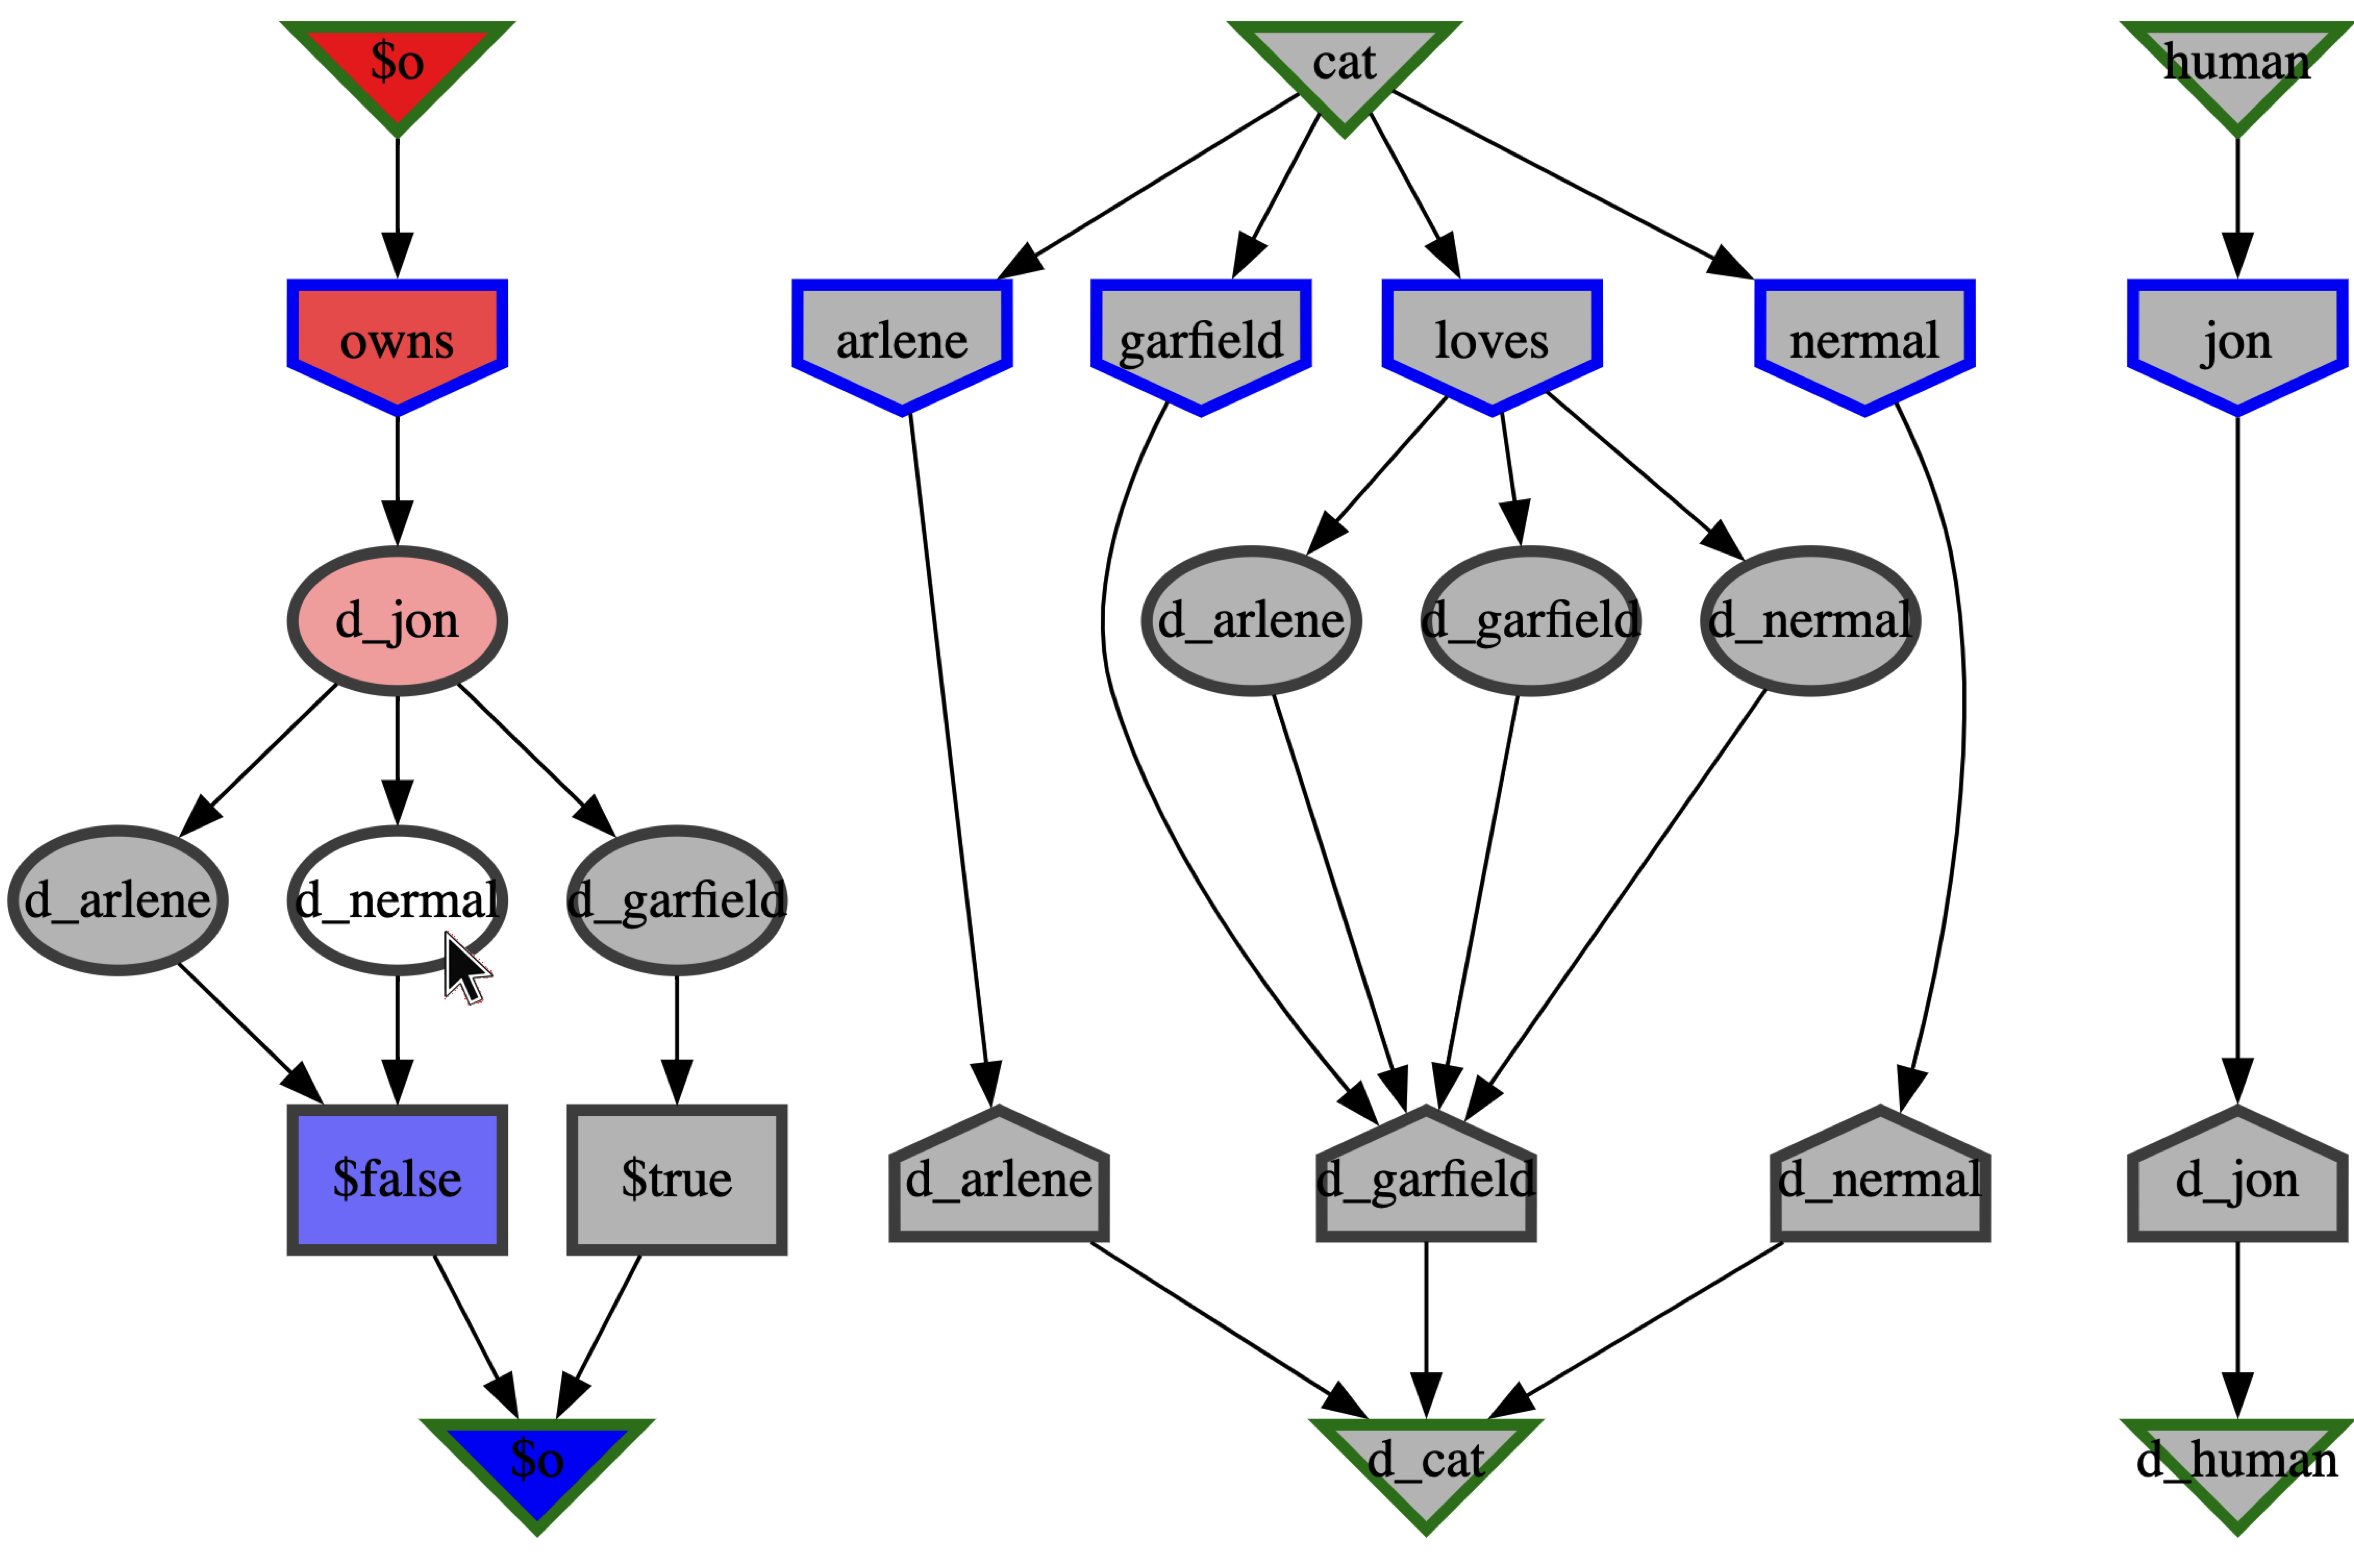
\includegraphics[width=\columnwidth]{TFF_Finite.s.IIV.pdf}
\caption{Visualization of the interpretation in Figure~\ref{TF0FiniteInterpretation}}
\label{TF0FiniteIIV}
\end{figure}

\begin{figure}[htbp]
\centering
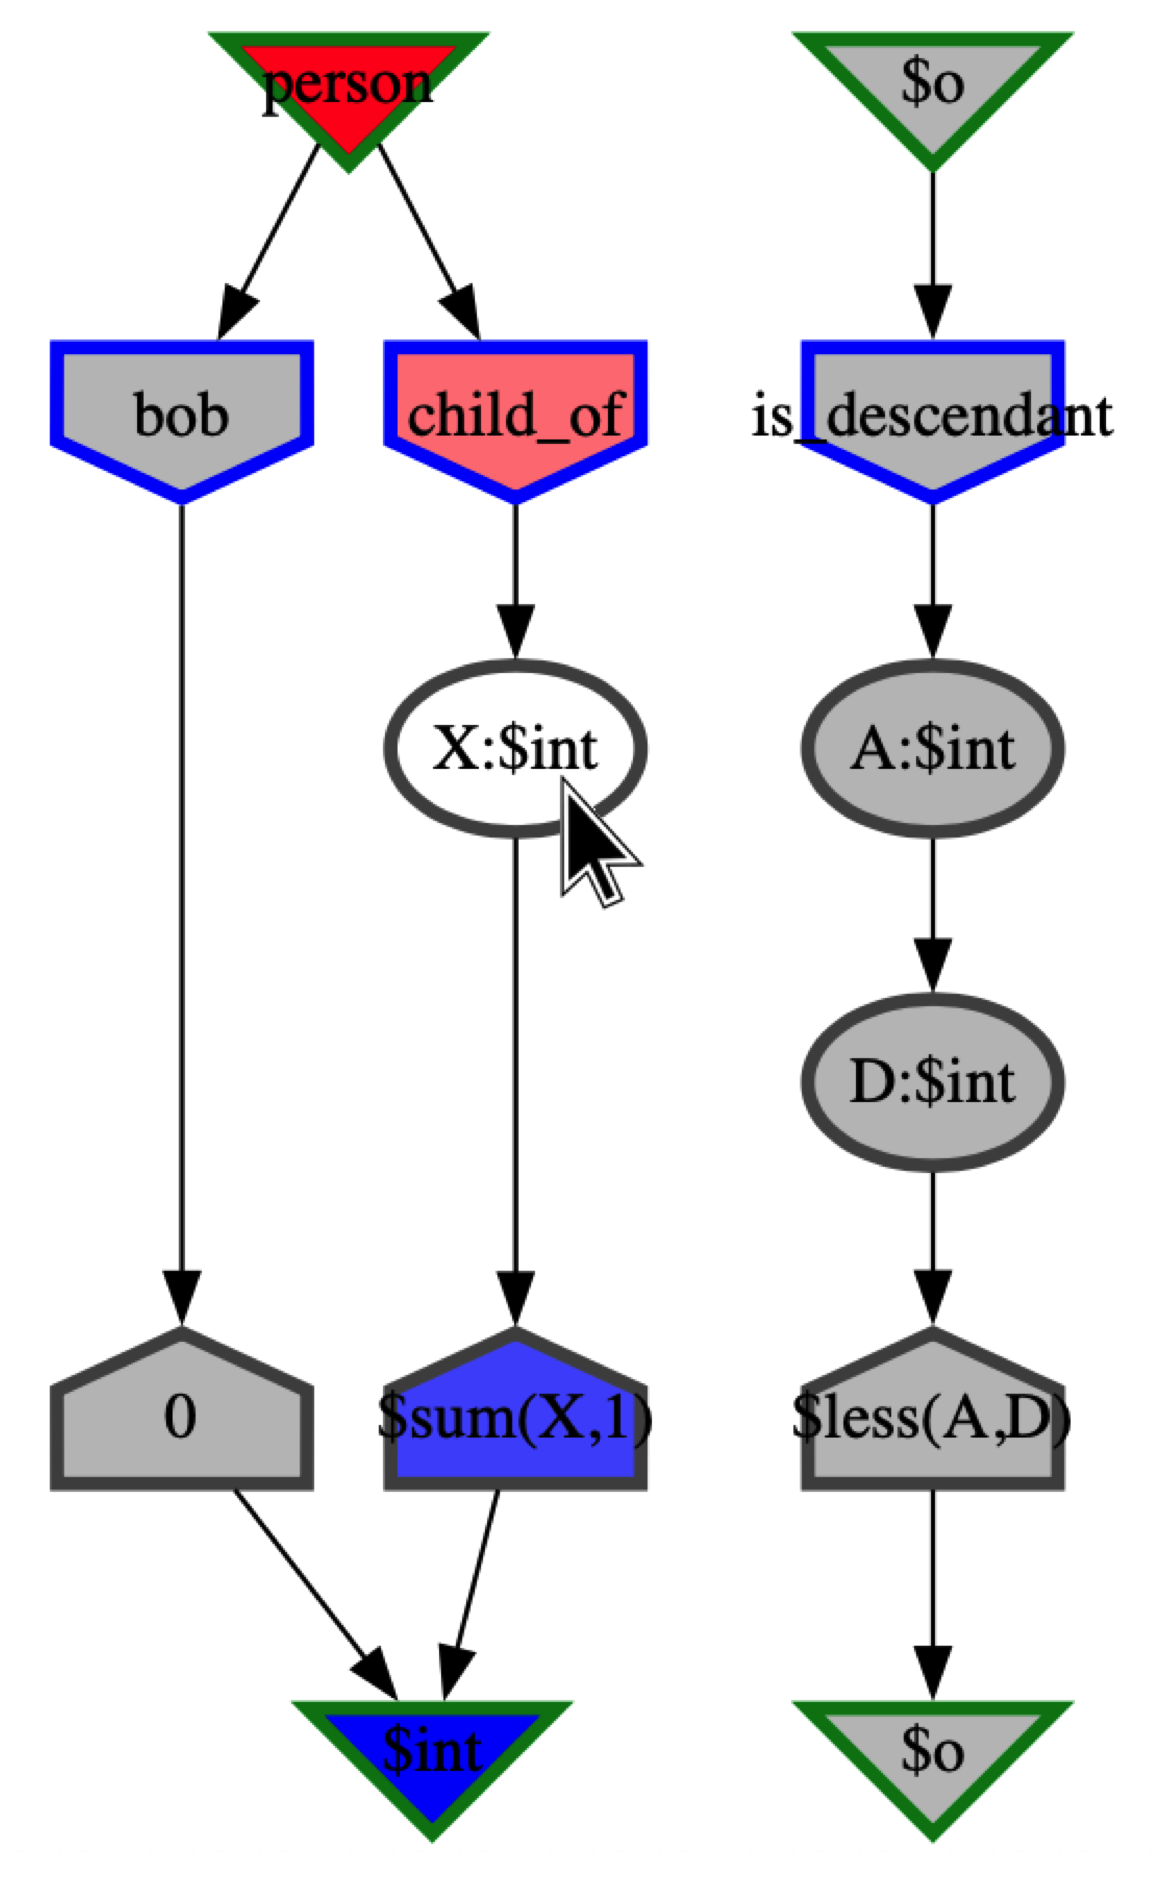
\includegraphics[width=0.45\columnwidth]{TFF_Integer.s.IIV.pdf}
\caption{Visualization of the interpretation in Figure~\ref{TF0InfiniteInterpretation}}
\label{TF0InfiniteIIV}
\end{figure}

%--------------------------------------------------------------------------------------------------
\section{Conclusion}
\label{Conclusion}

This paper describes the new TPTP format for representing Tarskian-style interpretations for
formulae in typed first-order logic, using the TPTP TF0 language.
It further describes a technique and an implemented tool for verifying models using this 
representation, and a tool for visualizing interpretations.
The research contributes to the advancement of automated reasoning technology for model finding, 
which has several applications, including verification.

Currently this work is being extended to Kripke interpretations for formulae in non-classical 
typed first-order logic \cite{SF+22}, using the TPTP NX0 language \cite{Sut22-IGPL}.
The tool to translate interpretation formulae to the format required for input to the IIV tool is 
being extended to infinite interpretations.
Further inspiration might also lead to improvements to IIV's visualizations, especially for more
complex infinite interpretations.

%--------------------------------------------------------------------------------------------------
\bibliographystyle{plain}
\bibliography{Bibliography.bib}
%--------------------------------------------------------------------------------------------------
\end{document}
%--------------------------------------------------------------------------------------------------
